\chapter{Test Strutturale}
\section{Adeguatezza e Copertura}
\paragraph{Thoroughness}
Come possiamo grantire la \textbf{scrupolosità} (completezza) dei test?
\\Per farlo dobbiamo rispondere alle seguenti domande:
\begin{itemize}
    \item \textbf{Quali} test dobbiamo generare?
    \item \textbf{Quanti} test dobbiamo generare?
    \item \textbf{Quando dobbiamo fermarci} a generare test?
\end{itemize}
In linea di principio, l'obiettivo dovrebbe essere quello di generare un'\textbf{adeguata} suite di test, vale a dire
una suite di test che, se il software sottoposto a test viene superato con successo, garantisca
una qualche proprietà del software stesso.

L'adeguatezza è quindi in principio una sorta di "assicurazione" sull'abilità della suite di test nel trovare difetti.

\paragraph{Non possiamo avere quello che vogliamo!}
Non possiamo garantire in nessun modo che una suite trovi tutti o alcuni dei difetti, e non possiamo garantire neanche che li trovi con alta probabilità:
\begin{center}
    \emph{«Testing can be used to prove the presence, not the absence, of errors»}
\end{center}
In sostanza nessun metodo di progettazione dei test fornisce alcuna garanzia sulla capacità di
scoprire difetti per le suite di test generate

\paragraph{Cosa Facciamo?}
Quindi come costruiamo una suite di test accettabile?
\\Potremmo continuare a generare test random e continuare a farlo finche non finiamo il tempo o il budget,
ma questa strategia non ci soffisfa euristicamente!

\subsection{Criteri di Adeguatezza}
Bisogna rinunciare all'idea disperata dell'adeguatezza come garanzia sul potere di rilevamento dei difetti,
e definire criteri euristici di adeguatezza simili alle regole di progettazione.

Molte discipline progettuali utilizzano regole di progettazione per valutare non se un progetto è
adeguato, ma se \emph{esso è inadeguato}.
L'idea è che un design che segue queste rule non è necessariamente adeguato, ma uno che non segue queste regole necessariamente sarà inadeguato!

\paragraph{Criteri pratici di (in)adeguatezza per i test}
Molti criteri di (in)adeguatezza per il testing derivano da osservazioni di buon senso su ciò che ci aspetteremmo come minimo da una suite di test.

\textbf{Ricorda} che questi criteri ci aiutano a capire perchè ci piace o non piace una suite di test,
ma soddisgarli (o no) non implica niente sull'effettiva abilità della suite nel trovare difetti!

\paragraph{Definizione di Criteri di Adeguatezza}
Diamo una definizione formale di criteri di adeguatezza:
\definizione{
    Un criterio di adeguatezza è un predicato che assume valore vero o falso
    per una coppia $<P,T>$, dove $P$ è un programma e $T$ è una suite di test.
    Se il criterio è $True$, diciamo che la suite è adeguata per il programma.
}
Un criterio di adeguatezza generalmente è fatto da sottopredicati chiamati \textbf{test obligations}.

Una suite $T$ soddisfa i criteri di adeguatezza per un dato programma $P$ \emph{se e solo se}:
\begin{itemize}
    \item Tutte le esecuzioni dei casi di test in $T$ su $P$ passano.
    \item Tutte le test obligations sono soddisfatte da almeno un test case nella suite.
\end{itemize}

\begin{center}
    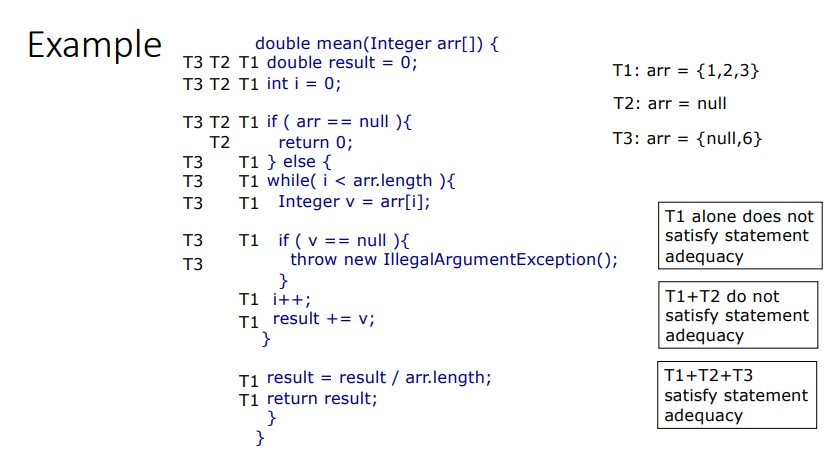
\includegraphics[width=.8\textwidth]{images/example_testing_adequacy.jpg}
\end{center}
In questo esempio abbiamo che i singoli test non riescono a soddisfare singolarmente i criteri di adeguatezza perchè non riescono a coprire l'intero codice.

%SLIDE 10

\section{Structural Testing}
A differenza del testing funzionale, in cui la completezza del test è giudicata sui requsiti senza tener conto del programma sotto esame,
nel testing strutturale viene giudicata la completezza del test in base alla struttura del programma.

Il test strutturale è anche chiamato "white/glass box testing", mentre quello funzionale è chiamato "black box testing".

Si noti che il testing strutturale consiste ancora nel testare il prodotto (codice) rispetto alle specifiche: cambia solo la misura della completezza!

\osservazione{I test confrontano \textbf{sempre} un programma con una specifica}

\subsection{Statement Coverage}
Per una suite di test T possiamo definire la \textbf{coverage} come la frazione di enunciati di P eseguiti da almeno un caso di test in T:
\[ C_{stmt} = \frac{\text{\# executed stmts}}{\text{\# stmts}} \]
Il test $T$ soddisfa il criterio di adeguatezza se e solo se $C_{stmt} = 1$.

%slide 15

%%Restart da slide 15 perché ho missato un commit.

\paragraph*{Unsatisfiable Test Obligations}
In alcuni programmi potrebbero esistere dei criteri di adeguatezza insoddisfacibili, come ad esempio 
alcuni statement non raggiungibili dai test.
Se non consideriamo questi elementi potremmo trovarci con delle suite che risultano inadeguate solo perché alcune obbligazioni non sono fisicamente soddisfacibili.

Abbiamo due approcci possibili a questo problema:
\begin{itemize}
    \item Rimuovere dai criteri di adeguatezza tutte le obbligazioni di test insoddisfacibili.
    \item Usare la covergae come una misura di quanto ci siamo avvicinati all'adeguatezza.
\end{itemize}

\subsection{Basic Blocks}
Si puó notare che se due statements sono in sequenza, eseguirne uno automaticamente implica eseguire anche l'altro.
Quindi possiamo considerare i \textbf{basic blocks}, dove le obbligazioni sono i blocchi del CFG\footnote{Control Flow Graph} del programma.

\definizione{Un Basic Block è una sequenza massima di istruzioni di programma contigue con un punto di ingresso e un punto di uscita.}